\documentclass%
%[handout]
{beamer}
% % % % % % % %
% % % % % % % %
% % % % % % % %
%IMPORTANT
%compiles with 
%pdflatex -shell-escape 
%IMPORTANT
% % % % % % % %
% % % % % % % %
% % % % % % % %
\mode<presentation>
{
\useinnertheme{rounded}
\useoutertheme{infolines}
\usecolortheme{orchid}
\usecolortheme{whale}
}

\usepackage[english]{babel}
\usepackage[latin1]{inputenc}
\usepackage{times}
\usepackage[T1]{fontenc}
\usepackage{../example-templates}
\usepackage{auto-pst-pdf}
\usepackage{pst-plot}

% Or whatever. Note that the encoding and the font should match. If T1
% does not look nice, try deleting the line with the fontenc.

\graphicspath{{../../modules/}}

\newtheoremstyle{partialproof}{3pt}{3pt}{}{}{}{.}{.5em}{}
\theoremstyle{partialproof} \newtheorem{partialproof}[theorem]{Proof.}
%\DeclareMathOperator{\diff}{d}
\newcommand{\diff}{\text{d}}
\setbeamertemplate{navigation symbols}{}

\includeonlylecture{1}

\newcommand{\lect}[3]{
  \date{#1}
  \lecture[#1]{#2}{#3}
}

\setbeamertemplate{footline}
{
  \leavevmode%
  \hbox{%
  \begin{beamercolorbox}[wd=.333333\paperwidth,ht=2.25ex,dp=1ex,center]{author in head/foot}%
    \usebeamerfont{author in head/foot}\insertshortauthor
  \end{beamercolorbox}%
  \begin{beamercolorbox}[wd=.333333\paperwidth,ht=2.25ex,dp=1ex,center]{title in head/foot}%
    \usebeamerfont{title in head/foot}\insertshorttitle
  \end{beamercolorbox}%
  \begin{beamercolorbox}[wd=.333333\paperwidth,ht=2.25ex,dp=1ex,center]{date in head/foot}%
    \usebeamerfont{date in head/foot}\insertshortdate{}
  \end{beamercolorbox}}%
  \vskip0pt%
}

% If you have a file called "university-logo-filename.xxx", where xxx
% is a graphic format that can be processed by latex or pdflatex,
% resp., then you can add a logo as follows:

%\pgfdeclareimage[height=0.8cm]{logo}{bluelogo}
%\logo{\pgfuseimage{logo}}

\begin{document}
\newcommand{\psHollowDot}[2]{
\pscircle*[fillcolor=white, linecolor=red](#1, #2){0.07}
\pscircle*[fillcolor=white, linecolor=white](#1, #2){0.04}
}
\newcommand{\psFullDot}[2]{
\pscircle*[fillcolor=white, linecolor=red](#1, #2){0.07}
}

\AtBeginLecture{%

\title[\insertlecture]{FreeCalc}
\subtitle{\insertlecture}
\author[FreeCalc]{}
\institute[UMass Boston]{University of Massachusetts Boston}
\date{\insertshortlecture}
\begin{frame}
  \titlepage
\end{frame}
}%

% begin lecture
\lect{\today}{Sample}{1}
% begin module inverse-function-ex5
\begin{frame}
\begin{example}%[Example 5, p. 388]
\begin{columns}[c]
\column{.5\textwidth}
\ \only<handout:0| -1>{%
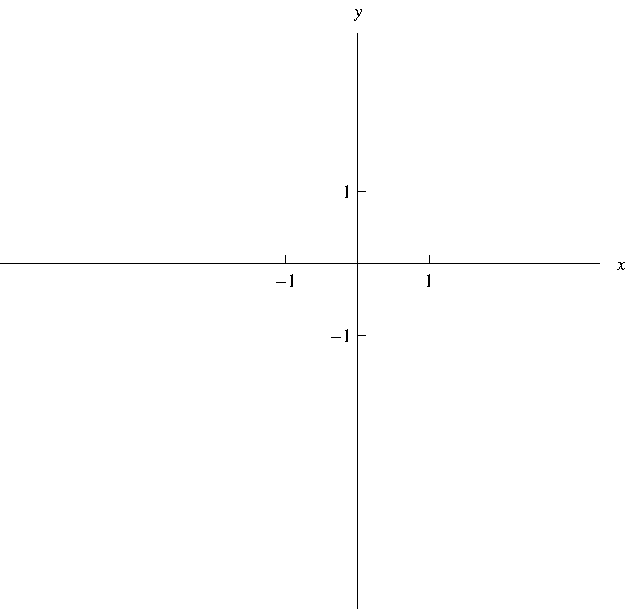
\includegraphics[height=4.5cm]{inverse-functions/pictures/07-01-ex5a.pdf}%
}%
\only<handout:0| 2>{%
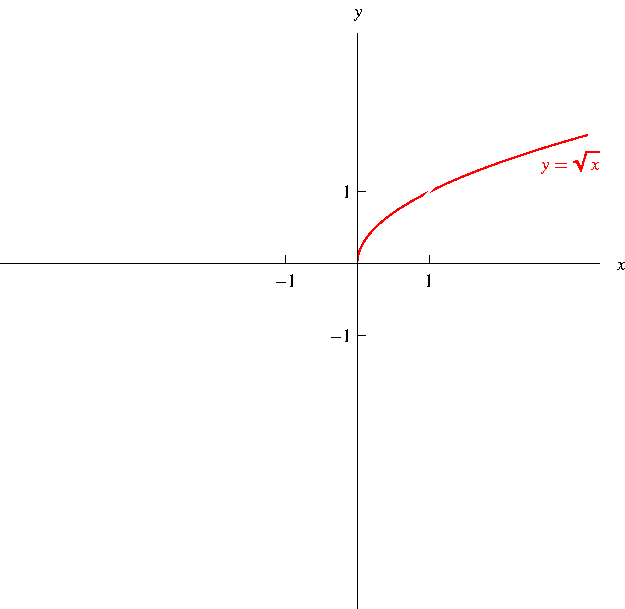
\includegraphics[height=4.5cm]{inverse-functions/pictures/07-01-ex5b.pdf}%
}%
\only<handout:0| 3>{%
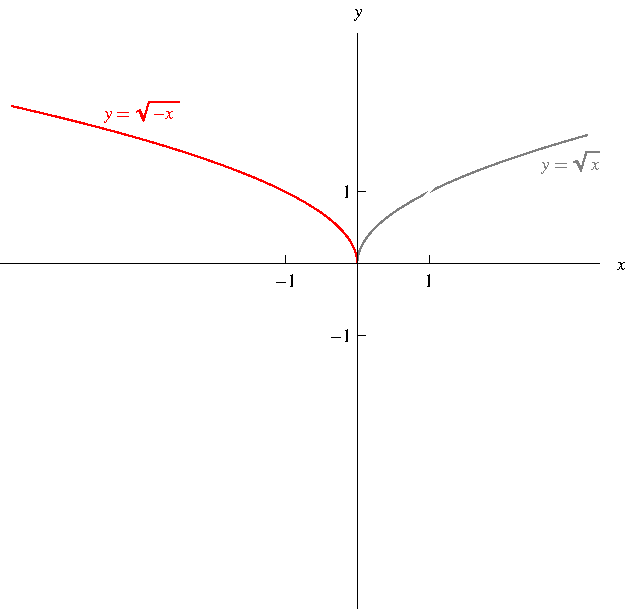
\includegraphics[height=4.5cm]{inverse-functions/pictures/07-01-ex5c.pdf}%
}%
\only<handout:0| 4>{%
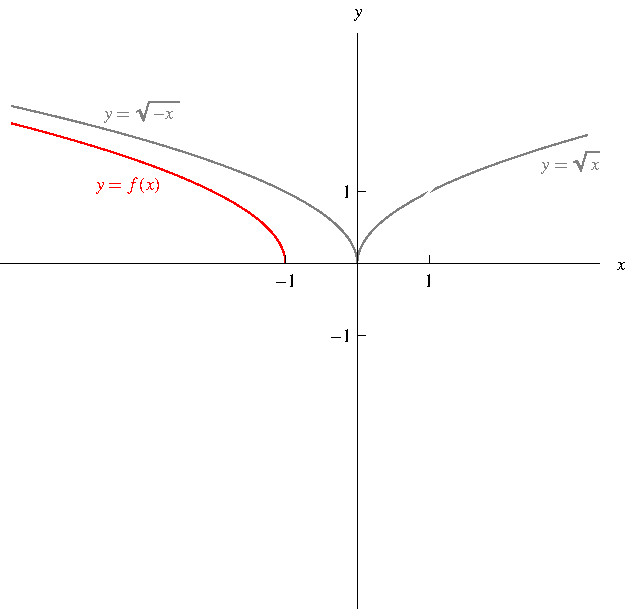
\includegraphics[height=4.5cm]{inverse-functions/pictures/07-01-ex5d.pdf}%
}%
\only<handout:1| 5->{%
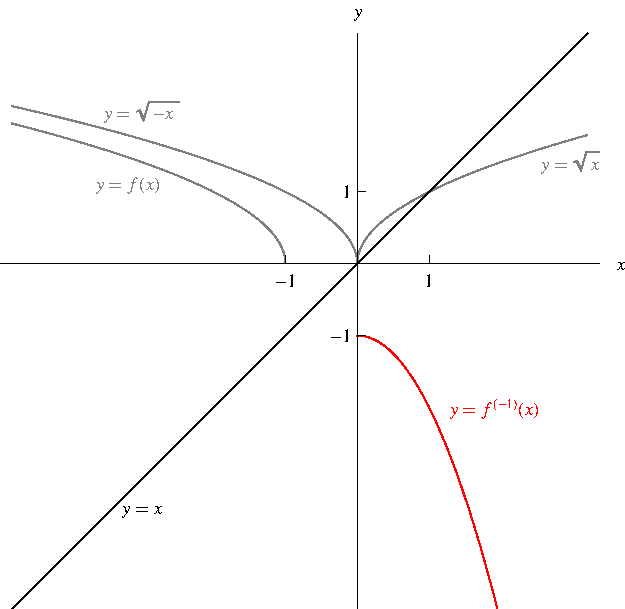
\includegraphics[height=4.5cm]{inverse-functions/pictures/07-01-ex5e.pdf}%
}%
\column{.5\textwidth}
Sketch the graph of $f(x) = \sqrt{-x - 1}$ and its inverse function.
\end{columns}
\begin{itemize}
\item<2->  First draw the graph of $y = \sqrt{x}$.
\item<3->  $y = \sqrt{-x}$ is the reflection of $y = \sqrt{x}$ in the $y$-axis.
\item<4->  $y = f(x) = \sqrt{-x - 1}$ is the shift of $y = \sqrt{-x}$ one unit to the left.
\item<5->  $y = f^{-1}(x)$ is the reflection of $y = f(x)$ in the line $y = x$.
\end{itemize}
\end{example}
\end{frame}
% end module inverse-function-ex5

% end lecture

\end{document}
